\chapter{Hosted Bytecode Interpreter}

A programming language interpreter executes programs in two steps.
First it parses the human readable source code, verifies its correctness and translates the code into a more efficient intermediate representation (IR) format.
The interpreter then picks up the translated program and executes it piece by piece.

Bytecode interpreters parse source program into bytecode, a highly compressed representation of the program.
The format of the bytecode is a form of virtual instruction set designed for this particular interpreter.
In the second step bytecode interpreters execute the bytecode as a sequence of virtual instruction one instruction at a time before finishing the last one.
Interpreters are also regard as virtual machines, since they emulate ``machines'' with their own virtual instruction sets.

In this Chapter, we go over performance overheads of bytecode interpreters and the classic techniques used to minimize these overheads.
Lastly, we introduce ModularVM~\cite{savrun2013, savrun2014}, a research JVM that automatically optimize the performance of hosted bytecode interpreters.

\section{Performance Anatomy of Bytecode Interpreters}

Bytecode interpreters execute bytecode one instruction at a time.
For each instruction, the interpretation consists of three steps~\cite{davis2003case}:
\begin{itemize}
  \item Instruction dispatch
  \item Operand access
  \item Performing the function of the instruction
\end{itemize}
Instruction dispatch includes fetching the next instruction, decoding the instruction and transferring program execution to the actual implementation of the instruction.
Operand access involves fetching operands required to perform the instruction from either a temporal operand stack or a virtual register file depending on the design of the virtual instruction set.
It also includes storing the computed result back to where temporal operands should be stored.
Subsequently in the last step the interpreter performs the actual computation.
For instance, if the instruction is addition of two numbers, the actually addition is performed in this step.

\begin{figure*}[th]
\centering
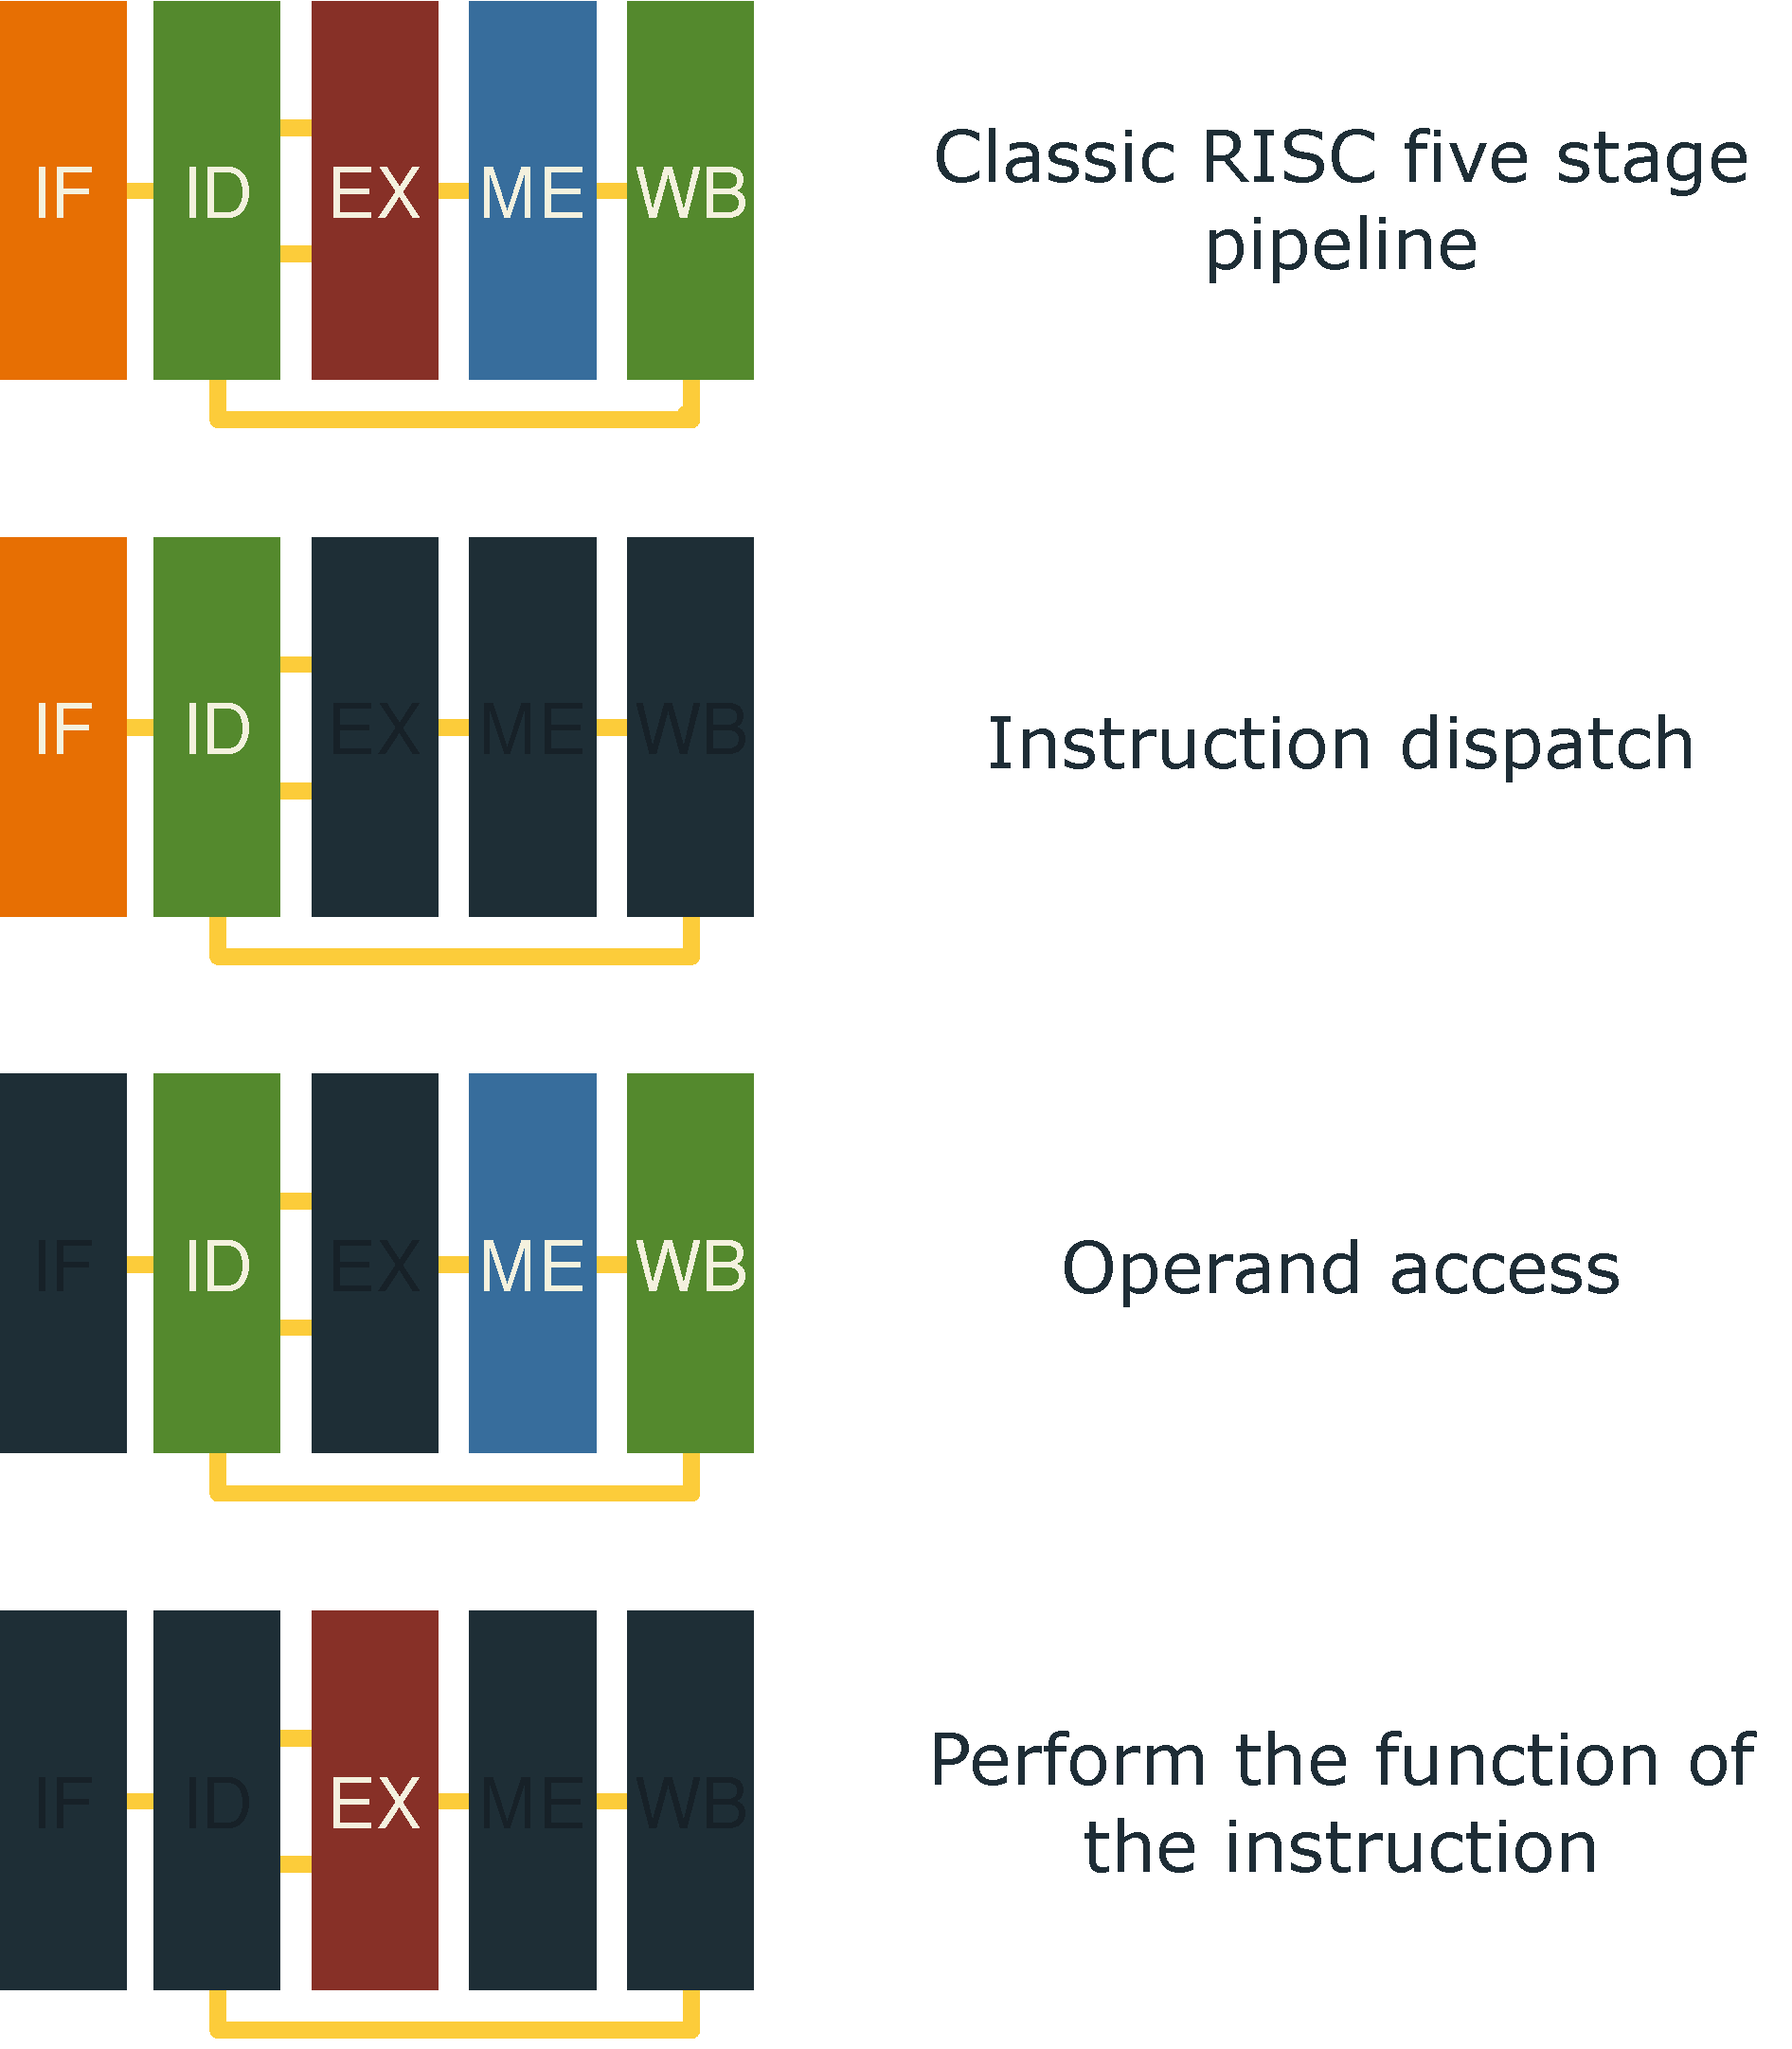
\includegraphics[scale=.25]{figures/ch2-risc-pipeline.pdf}
\caption{Interpretation costs of bytecode interpreters}
\label{fig:interpretation-cost}
\end{figure*}

An interesting way to further illustrate the purpose of each interpretation step
from the angle of a virtual machine is to correlate each step with the stages in a classic reduced instruction set computer (RISC) pipeline.
Figure~\ref{fig:interpretation-cost} illustrates the five stages in a classic RISC pipeline:
instruction fetch (IF), instruction decode (ID), execute (EX), memory access (ME) and write back (WB).
The instruction dispatch step in bytecode interpreters is similar to instruction fetch and decode stages in RISC.
We can correlate the late stage of instruction decode, memory access and write back in RISC to operand access in an interpreter.
Since these are the pipeline stages that prepare the operands for the computing unit and stores the end result back to either a register or memory address.
The interpreter step that performs the function of the instruction works exactly as the execute stage in RISC, which performs the actual computation.

The cost of running a hosted program on an interpreter consists of the costs of performing each of the three steps we described above.
Among those steps, instruction dispatch and operand access does not directly contribute to the actual work of the hosted program.
The less time the interpreter spend in these two steps, the more time the interpreter spend in doing the actual work.
Therefore, an efficient bytecode interpreter must encompass techniques that optimize instruction dispatch and operand access.
